
\documentclass{sig-alternate}
\usepackage{graphicx} 
\usepackage{bussproofs} 
\usepackage{listings}
\usepackage{color}
% This is the "centered" symbol
\def\fCenter{{\mbox{\Large$\rightarrow$}}}

\definecolor{LightGrey}{rgb}{0.9,0.9,0.9}
\lstset{numbers=left, numberstyle=\tiny, numbersep=2pt, basicstyle=\ttfamily\small, tabsize=2, backgroundcolor=\color{LightGrey}}

% Optional to turn on the short abbreviations
\EnableBpAbbreviations

% \alwaysRootAtTop  % makes proofs upside down
% \alwaysRootAtBottom % -- this is the default setting

\begin{document}

\title{New Ideas and Emerging Results Track: Towards Unifying, Functional Programing, Rule-Based Programming, and Event-Based Programming}

\numberofauthors{1}
\author{
\alignauthor
Renaud Pawlak\\
       \affaddr{LISITE-ISEP}\\
       \affaddr{28 rue Notre-Dame des Champs}\\
       \affaddr{Paris, France}\\
       \email{renaud.pawlak@isep.fr}
}
\date{30 July 1999}

\maketitle
\begin{abstract}
In this paper, we discuss rule-based programming with a new language called INI, which we created to evaluate rule-based oriented programming in terms of code simplicity, quality, and maintainability. INI takes inspiration from existing rule-based languages, mostly from languages permitting rewriting rules, but also from functional languages allowing imperative style programming. We shortly and informally present the INI syntax and semantics, and, using some simple examples, we show how to use INI for rule-based programming. We discuss rule-oriented code and we show that INI also allows to fall into functional programming style in a consistent way. Our claim, and the novelty here, is that rule-based programming mixed with functional programming here leads to more maintainable code, since it forces the programmers to explicitly write the pre-condition upon which some behavior shall be executed. In addition, it simplifies the code by replacing most imperative control-flow constructs such as various looping constructs and if then else constructs, with a consistent and unique rule construct. Last but not least, we show that our programming model allows for consistent integration of event-based programming through event-triggered rules. This event-based model allows for intuitive multithreaded programming, which makes it suitable for many types of applications such as embedded application and server applications. 
\end{abstract}

% A category with the (minimum) three required fields
\category{H.4}{Information Systems Applications}{Miscellaneous}
%A category including the fourth, optional field follows...
\category{D.2.8}{Software Engineering}{Metrics}[complexity measures, performance measures]

\terms{Rule-based Programming}

\keywords{Programming Language, Code Quality, Rule-based Programming, Functional Programming}

\section{Introduction}

In this paper, we present INI, a rule-based programming language. In INI, all functions are defined with rules, i.e. guarded actions. An action is executed only if its guard is evaluated to true in the context of the function. Also, an action will continue to be evaluated while its guard is true. This specificity can be found in rewriting-based languages [...]. However, INI is not intended to deal only with structure rewriting, since the actions may have classical behaviors and side-effects, like in typical imperative languages. 

Thus, INI allows rule-based programming style, which will be studied in this paper. First, we will see that rule-based programming allows for some algorithms to be implemented quite straightforwardly, and that it enforces the programmer to declare pre-conditions, thus leading to better programming style and code safety. Second, we will see that rule-based programming leads to straightforward asynchronous and multithreaded programming, thanks to event-triggered rules. Third, we will show that rule-based programming is not incompatible with functional programing, since INI allows the programmer to fall back on this style of programming when rule-based programming is not well adapted to the problem to solve. Finally, we will shortly present the INI implementation, which is built on Java and allows easy extension, through bindings, but also with the definition of new built-in functions and events. A small case study will also be discussed.

\section{INI in a Nutshell}

In order to discuss our programming model, we first present INI very shortly. A complete reference manual is available at [...]

\subsection{Overview}

INI is a programming language where all functions are defined with rules. A rule is defined with a guard and an action. The action will be executed only if the guard is evaluated to \texttt{true} in the context of the function. In other words: when the guard is passed, it triggers the evaluation of the action. The action is a list of sequential statements including variable assignments, function invocations, and return statements. These statements are similar to imperative language ones, except that they do not allow any control flow language constructs such as \emph{ifs} or \emph{loops}. In INI, a function does not terminate before all its rules' guards are evaluated to \texttt{false}, except when an action explicitly forces the function to end (with a return statement or an error). 

Syntactically, a function is written as:

{ \small \begin{verbatim}
function <name>(<parameters>) { 
  <guard1> { <statements> }
  <guard2> { <statements> }
  ...  
  <guardN> { <statements> }
}
\end{verbatim} }

Guards are either an event expression, or a logical expression, or both:

{ \small \begin{verbatim}
<guard> := <logical_expr>
         | <event_expression>
         | <event_expression> <logical_expr>
\end{verbatim} }

Logical expressions are formed of variable accesses, function invocations, and literals (strings, numbers, ...), composed together with classical logical operators (\texttt{\&\&} (and), \texttt{||} (or), \texttt{!} (not)) and/or comparison operators (\texttt{==}, \texttt{!=}, \texttt{>}, \texttt{>=}, \texttt{<}, \texttt{<=}). INI also defines a match operator ($\sim$) that allows for regular expression matching on strings and for type matching, similarly to the match construct in OCAML. In guards, logical expression must be evaluated to \texttt{true} to allow the evaluation of the rule's action. If a logical expression is not specified (event-only expression), it is equivalent to an always-true expression.

Event expressions are more original since they allow the programmer to specify that the rule evaluation is triggered upon one or several events. Events start with \texttt{@}, have a name, and can take parameters. In an event expression, events can be composed with two main temporal operators: sequentiality (\texttt{;}) and co-incidence (\texttt{\&}). The expression \texttt{@a(..);@b(..)} means that the \texttt{@a} and \texttt{@b} events must happen in that order, while \texttt{@a(..)} \texttt{@b(..)} means that \texttt{@a()} and \texttt{@b()} must happen in any order. \texttt{@a(..)\&@b(..)} means that both event must happen at the same time, which implies that at least one of the events has a duration. When a guard contains an event expression, it means that the rule is event-trigerred and is evaluated asynchronously whenever the event or events occur in the way specified by the expression. INI provides two special events for function initialization and termination: \texttt{@init}, which occurs when the function evaluation starts, i.e. before any other events or rules, and \texttt{@end}, which occurs once the function ends, that is to say when no rules can apply anymore (all the guards are evaluated to \texttt{false}). For a given function, \texttt{@init} and \texttt{@end}-triggered rules are executed only once and take no parameters.

\subsection{Example}

To illustrate INI, let us show a simple example that implements some sort of infinite ping-pong game between two rules.

\begin{lstlisting}
function ping_pong() {
	@init() {
		v=1
	}
	v == 2 {
		println("pong")
		v = 1
	}
	v == 1 {
		println("ping")
		v = 2
	}
}
\end{lstlisting}

When entering \texttt{ping\_pong}, INI first evaluates the \texttt{@init}-trigerred rule at line 2 that initializes a \texttt{v} variable to 1. Then, INI sequentially tries out all the rules of the function in their declaration order. Here, the guard at line 5 evaluates to \texttt{false}, but the one at line 9 evaluates to \texttt{true}, thus triggering the evaluation of the action that prints out \texttt{"ping"} (line 10) and sets \texttt{v} to 2 (line 11). After that, remember that the function will not terminate before all the guards evaluate to \texttt{false}. So, since line 5 now evaluates to \texttt{true}, INI evaluates the rule that prints out \texttt{"pong"} (line 6) and resets \texttt{v} to 1 (line 7). This action obviously triggers again the other rule, thus starting the endless ping-pong game over again. Note that the rules declaration order is not important here. Any other rule order will give the same result. That's because the guards are \emph{disjoint}.



\section{Rule-Based Programming}

\subsection{Programming the Behavior}

From a behavioral perspective, what is interesting about the Rule-Based Paradigm is that it clearly shows the conditions upon which some code can be executed. Indeed, guards can be seen as precondition for the actions. Because of this, the code representation naturally shows the states and transitions of the functions, if any. For instance, if we take again the \texttt{ping\_pong} function, it is pretty straightforward to see that it corresponds to the following state machine:

\begin{figure}[htbp]
\begin{center}
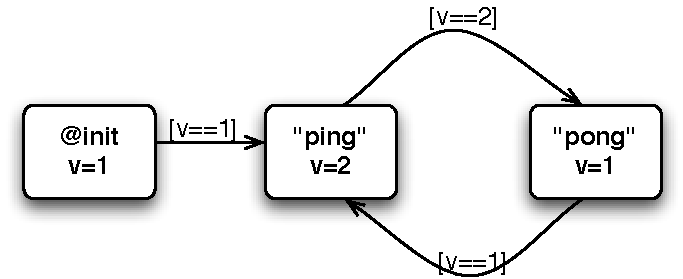
\includegraphics[scale=0.6]{ping_pong_sm.pdf} 
\caption{The \texttt{ping\_pong} function state machine}
\label{default}
\end{center}
\end{figure}

To show are more complicated example, the following code reads some text from the keyboard and writes \texttt{"hello"} to a file named after the read text. Also, the file is not written if it already exists on the file system.

\begin{lstlisting}
function write_hello() {
	!fname {
		print("enter a file name> ")
		fname = read_keyboard()
		f_exists = file_exists(fname)
	}
	fname && !f_exists {
		fprint(fname,"hello")
		clear(fname)
	}
	fname && f_exists {
		println("'"+fname+"' already exists")
		clear(fname)
	}
}
\end{lstlisting}

The three rules at lines 2, 7, and 11 show all the possible transitions depending on the variables states. Note that \texttt{!fname} is \texttt{true} if \texttt{fname} is undefined, \texttt{false} otherwise: within a guard, a non-boolean variable evaluates to a boolean value depending on its definition state (defined/undefined). Note also the use of the \texttt{clear(fname)} built-in functions at lines 9 and 13 that reset the \texttt{fname} variable and go back to the initial rule of line 2. Finally, an analysis of the function allows us to build the following state machine, which shows the possible transitions.

\begin{figure}[htbp]
\begin{center}
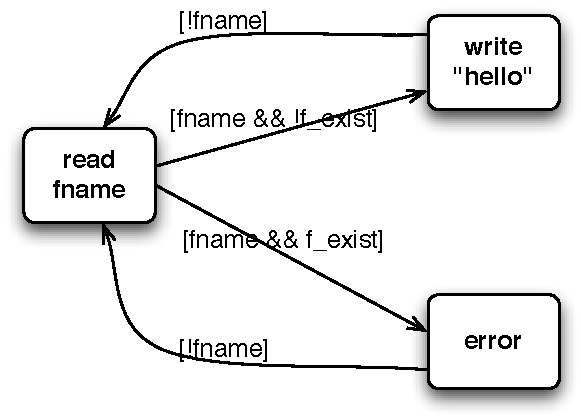
\includegraphics[scale=0.6]{read_sm.pdf} 
\caption{The \texttt{write\_hello} function state machine}
\label{default}
\end{center}
\end{figure}

Similarly to the \texttt{ping\_pong} function, the \texttt{write\_hello} function never terminates. This may seem ackward to programmers used to functional programming, where non-termination means infinite recursion. It is however completely normal behavior for interactive programs such as servers, data exchange protocols, batch jobs, etc. In such kinds of programs, it is actually important that the program never terminates and that the entire state space (possibilities) is clearly handled by the program. Our first experiments with rule-based programming show that the code for such interactive programs looks simple and intuitive to understand. 

\subsection{Asynchronism and multithreading}

Most interactive programs require the use of asynchronous events and parallelism. For instance, a batch job may need to perform a given task at a given time of the day, a server will require several clients to be served in parallel, and so on. For such cases, INI allows for event-triggered rules, which enable event-based programming with implicit parallelism. Such event triggering is also found in some specific languages used for programming complex and highly interactive systems, such as languages used in video games and robotics, for example Urbiscript [...]. 

The advantage of INI over other event-based languages, is that its rule-based programming model makes it possible to cleanly and intuitively integrate events as part of the guards. Example of INI built-in events are \texttt{@every(time)}, which is triggered at regular time intervals given in milliseconds, \texttt{@cron("crontab expression")}, which allows for the scheduling of events at specific time and dates (using an underlying crontab engine [...]), \texttt{@error(message)}, which is triggered when an error occurs or is thrown by the program, and last but not least, \texttt{@update(var1, var2, ... varN)}, which is triggered when one of the given variables is updated by the program (with an assignment).

Using the \texttt{@update} event, we have programmed an HTTP server prototype with INI. It uses the socket API. The \texttt{socket\-\_accept(s)} at line 6 is a blocking call that waits until a client connects to the server socket created at line 3. At this point, instead of dealing with the connection right after the \texttt{socket\_accept(s)} call returns, we simply set the returned socket to the \texttt{c} variable, that we observe using the \texttt{@update(c)} event at line 9. 

\begin{lstlisting}
function start_http_server(port, handler) {
	@init() {
		s = socket_server(port)
		println("Server started on "+port)
	}
	s { 
		c = socket_accept(s)
	}
	@update(c) {
		// handle http requests here
		client = socket_address(c)
		...
	}	
}
\end{lstlisting}

INI events are executed in separate thread, within the function context, thus enabling implicit parallelism. This way, our HTTP server can handle several clients in parallel. Using this technique, we have also programmed a prototype of an M2M gateway that reads some sensors, stores the value in some files, and every day at midnight (\texttt{@cron("0 0 * * *")} event), it creates a zip and sends it by FTP to a server.

\section{Functional Programming}

As explained before, rule-based programming is well suited to program highly interactive systems. However, it is sometimes more appropriate to use a functional-programming style, especially when a function needs to return the result of a calculation, and even more when this calculation is easy to express in a recursive manner.

\subsection{Functional v.s. Rule-Based Style\label{subsec:functional_style}}

The INI programming model makes it possible to switch from a rule-based paradigm to a functional paradigm so that both styles can consistently cohabit within the same program. For instance, the following code shows both versions of a factorial function. 

\noindent
\begin{minipage}[t]{0.5\linewidth}\centering
\begin{lstlisting}[numbers=none]
function fac(n) {
	@init() {
		f=1
		i=1
	}
	i <= n {
		f=f*i++
	}
	@end() {
		return f
	}
}
\end{lstlisting} 
\end{minipage}
\begin{minipage}[t]{0.5\linewidth}\centering
\begin{lstlisting}[numbers=none]
function fac(n) {
	n==1 {
		return 1
	}
	n > 1 {
		return n*fac(n-1)
	}
}
\end{lstlisting}
\end{minipage}

On the left, we can see the rule-based version, that defines 3 rules:

\begin{enumerate}
\item an initialization \texttt{@init}-triggered rule that defines and initializes a variable to store the result (\texttt{f}) and a variable to store the current integer to multiply (\texttt{i}).
\item a rule that multiplies the result by the current integer \texttt{i} and increments it, guarded with the condition that \texttt{i} is lower or equal to the number \texttt{n} we want to calculate the factorial of. Due to the INI execution semantics, this rule will continue to apply until \texttt{i<=n} becomes \texttt{false}, which eventually happens since \texttt{i} is incremented at each rule execution (\texttt{i++} expression). Once \texttt{i} equals to \texttt{n}, there are no rules to be executed anymore in the function.
\item a termination \texttt{@end}-triggered rule that returns the calculated result \texttt{f}.
\end{enumerate}

The functional version on the right-hand side is quite simpler since factorial calculation is easy to define recursively. Thus, we can define one rule that recursively uses \texttt{fac(n-1)} to calculate \texttt{fac(n)} for \texttt{n>1}, and a non-recursive rule for \texttt{n==1}, that simply returns 1 (the factorial value for \texttt{fac(1)}) for terminating the recursion. Note that each rule causes the function to end immediately because of the \texttt{return} statement.

Similarly to imperative style v.s. functional style, both rule-based and functional styles have advantages and drawbacks depending on what needs to be done. So, we think that it is good that both styles consistently cohabit within the same programming model. 

\subsection{Type Matching\label{subsec:type_matching}}

In order to fully allow functional programming style, it is import to enable ways to construct algebraic types, that allow the programmers to define complex structures. For the program to be well-typed when using these structures, INI supports a match operator, which is similar to the match construct in advanced functional languages such as CAML and Haskell. To demonstrate the use of such types, we show an INI program that allows the construction of algebraic expressions, and their evaluation with an \texttt{calc} function. This function uses the match operator within the rules guards to switch to the right action depending on the actual type constructor. 

\begin{lstlisting}
type Expr = Number[value:Float]
          | Plus[left:Expr,right:Expr]
          | Mult[left:Expr,right:Expr]
          | ...

function main() {
	@init() {
		// construct (3.0*2.0)+1
		expr = Plus[
			left=Mult[
				left=Number[value=3.0],
				right=Number[value=2.0]],
			right=Number[value=1.0]]
		println(expr+" = "+calc(expr))
	}
}

function calc(expr) {
	expr ~ Number[value] {
		return expr.value
	}
	expr ~ Plus[left,right] {
		return calc(expr.left)+calc(expr.right)
	}
	expr ~ Mult[left,right] {
		return calc(expr.left)*calc(expr.right)
	}
	...
}
\end{lstlisting}

Note that INI also support other features coming from functional programming such as higher order functions. Although not proven, we do not see any reason yet why rule-based programming could not cohabit with functional programing. It is however not the main goal of INI to fully support functional programing. The next section relates much more important goals.

\section{Typing and Validations}

In this section, we present the most important feature of INI: the typing, which is implemented with a type inference algorithm, and the validations, which is work in progress to statically check that the program is correct. 

\subsection{Motivations}

Formal methods propose techniques to prove that the program behaves accordingly to some formal specifications. Formal methods can be categorized in proof-based frameworks, such as B and Coq, and model-checking tools, that try to cover the entire state-space to ensure some properties. The difficulties with formal methods is that they require the formal modeling of the programs, which is a hard and expensive task to achieve. Other validation techniques called static analysis techniques start from the program actual code to check that it is correct. Static analysis tools can be seen as extra compilation stages that go far beyond typing. Partial evaluation [...], control-flow analysis [...], symbolic evaluation (Javapath) [...], points-to analysis [...] are examples of static analysis techniques that can be used to automatically detect programming mistakes such as the use of undefined variables, out of bounds variables, unused variables and/or code.

Although theorically 

\subsection{Type inference}

INI provides \emph{type inference} [...], so that the programmer does not need to declare any type (except in some cases as we will see later). For instance, the \texttt{i=0} statement will define the \texttt{i} variable with an \texttt{Int} type. If the programmer tries to set the type of \texttt{i} to any other type within the \texttt{i} definition scope, (for instance with the \texttt{i=0.0} statement that assigns i with a \texttt{Float} type) the INI type checker will raise a type mismatch error. Following the same type inference principles, accessing a variable with the square brackets map access construct will automatically define the type of the variable to be a map. For instance, the \texttt{l[i]} expression tells INI that \texttt{l} is of type \texttt{Map(Int,T)} (i.e. a list of \texttt{T}), where \texttt{T} can be any type. 

As said in Section \ref{sec:counting_occurences_in_a_list}, most types in INI are calculated with the type inference engine, which allows the programmers to say very few about the typing. The kernel of this type inference is based on a Herbrand unification algorithm, as depicted by Robinson in \cite{robinson1965}. The typing algorithm is enhanced with polymorphic function support, abstract data types (or algebraic types) support, and with internal sub-typing for number types.

Thus, INI works with the following steps:

\begin{enumerate}
\item the parser constructs the AST;
\item an AST walker constructs the typing rules that should be fulfilled for each AST node and add them to a constraint list;
\item a unification algorithm is run on the type constraints, if conflicts are detected, they are added to the error list;
\item if errors are found, they are reported to the user and INI does not proceed to the execution phase.
\end{enumerate}

\subsection{Rule-based validations}

\section{Conclusion and Future Work}

In this paper, we discuss rule-based programming with a new language called INI, which we created to evaluate rule-based oriented programming in terms of code simplicity, quality, and maintainability. INI takes inspiration from existing rule-based languages, mostly from languages permitting rewriting rules, but also from functional languages allowing imperative style programming. We shortly and informally present the INI syntax and semantics, and, using some simple examples, we show how to use INI for rule-based programming. We discuss rule-oriented code and we show that INI also allows to fall into functional programming style in a consistent way. Our claim, and the novelty here, is that rule-based programming mixed with functional programming here leads to more maintainable code, since it forces the programmers to explicitly write the pre-condition upon which some behavior shall be executed. In addition, it simplifies the code by replacing most imperative control-flow constructs such as various looping constructs and if then else constructs, with a consistent and unique rule construct. Last but not least, we show that our programming model allows for consistent integration of event-based programming through event-triggered rules. This event-based model allows for intuitive multithreaded programming, which makes it suitable for many types of applications such as embedded application and server applications. 


%\bibliographystyle{plain}	% (uses file "plain.bst")
%\bibliography{ini_manual}		% expects file "ini_manual.bib"

\end{document}

